\chapter{Introduction}
%\chapter{Einleitung}
\label{sec:introduction}

general motivation for your work, context and goals: 1-2 pages

\begin{itemize}
\item \textbf{Context:} make sure to link where your work fits in
\item \textbf{Problem:} gap in knowledge, too expensive, too slow, a deficiency, superseded technology
\item \textbf{Strategy:} the way you will address the problem 
\end{itemize}


\section{Sample Section}

The following samples explain how to insert cross-references, figures and tables, how to set math, algorithms and program code, how to add references, and how to use acronyms.


\subsection{Cross References}
\label{sec:cross-ref}

Use the \verb|\label| and \verb|\cref| commands for cross references, e.g.\ to \cref{sec:cross-ref}. 

\subsection{Figures}

\Cref{fig:setup0} shows the distribution of the nodes in the sample setup at time $t=0$, as well as the initial coverage with a sensing radius of \SI{30}{\metre} and the communication graph for a communication range of \SI{50}{\metre}.

\begin{figure}
	\centering
	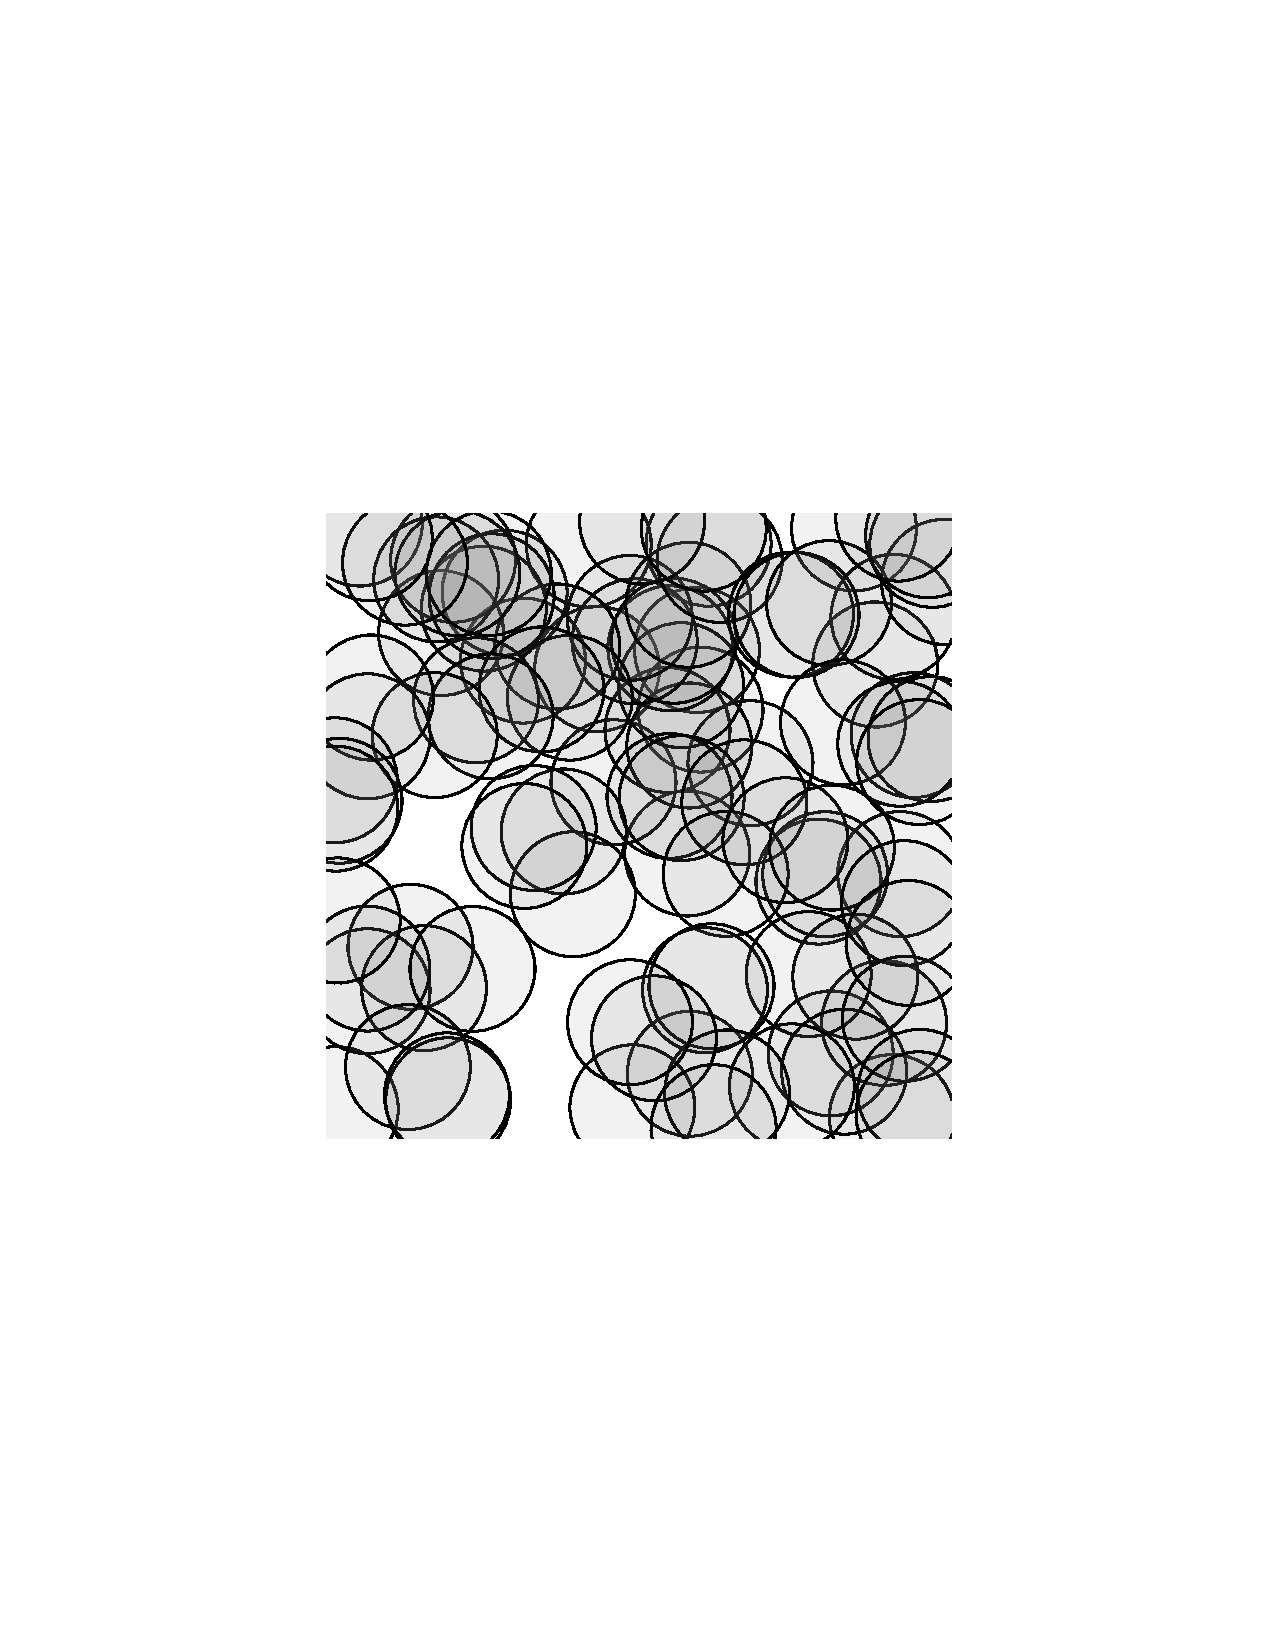
\includegraphics[width=0.3\textwidth]{figures/coverage-30--0-static1}
	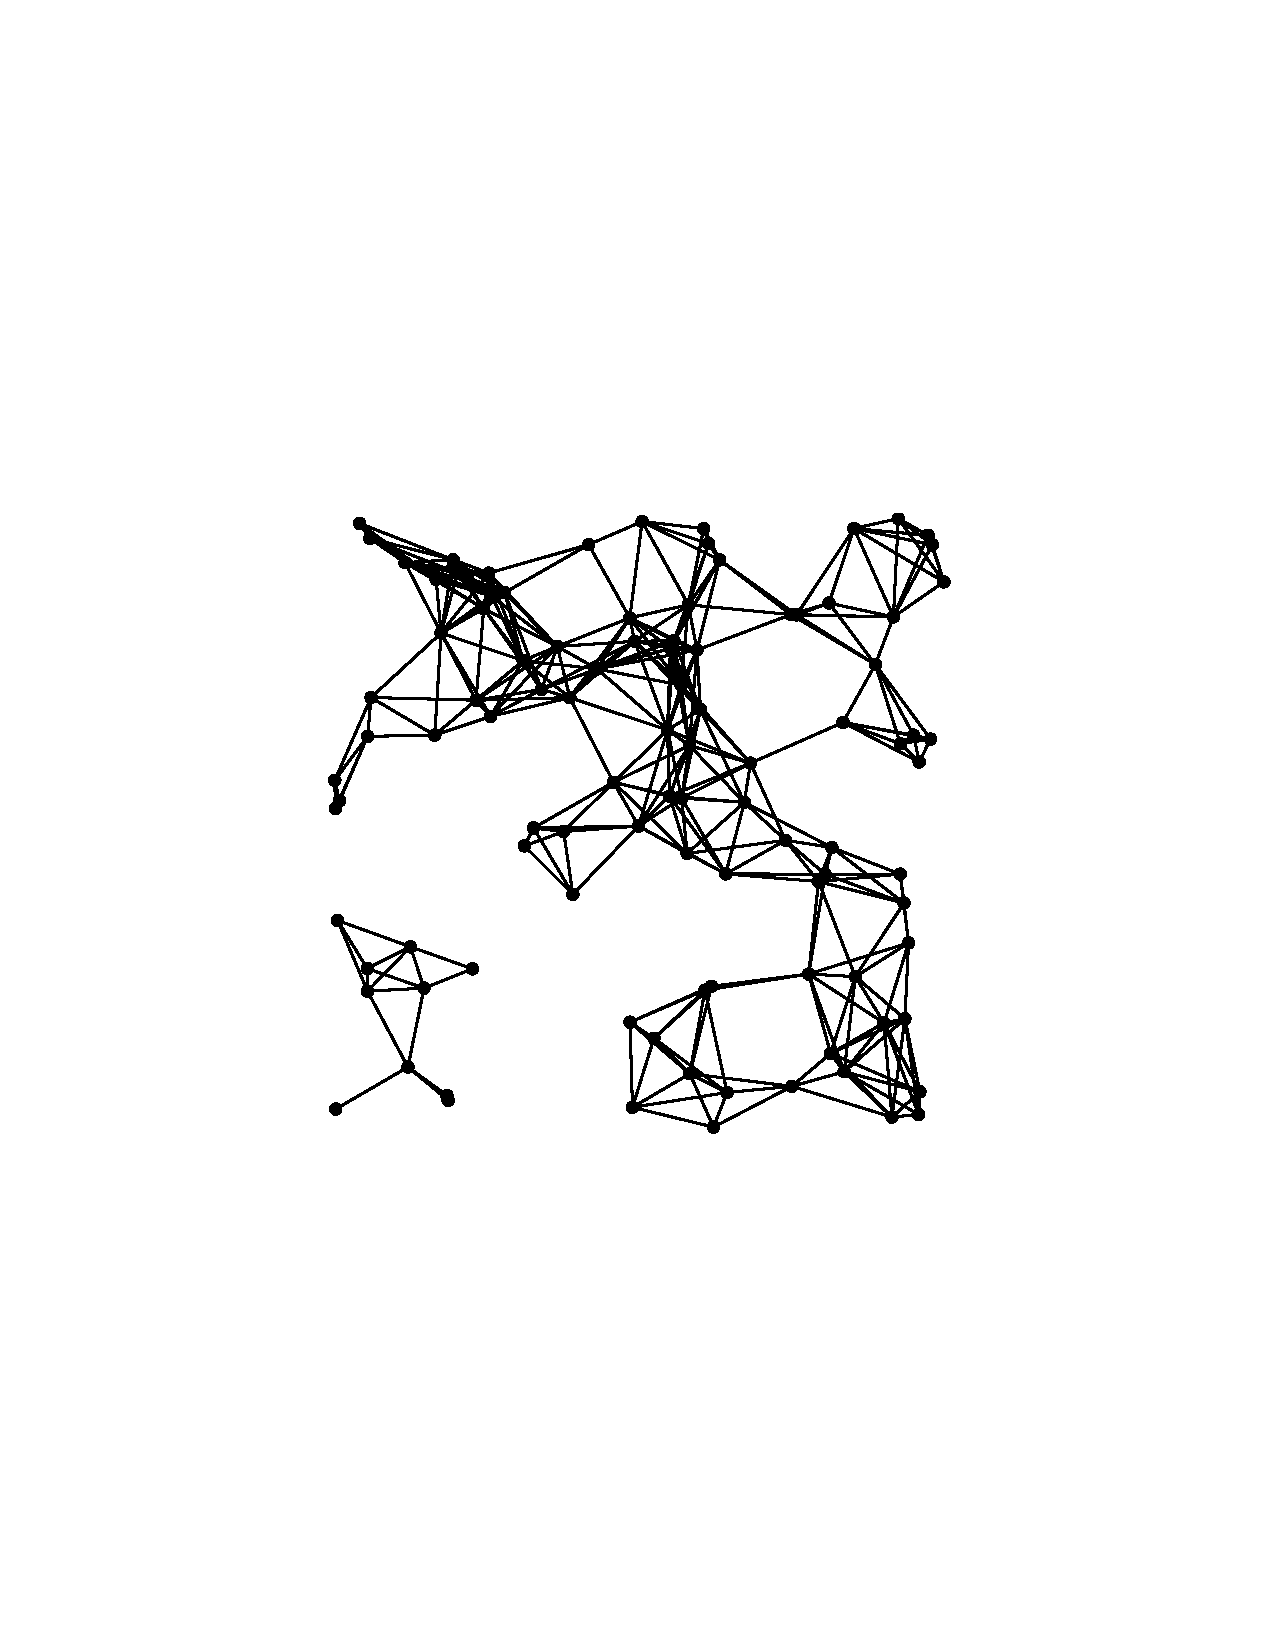
\includegraphics[width=0.3\textwidth]{figures/connectivity-50-0-static1}
	\caption{Coverage and connectivity for a sample replication at time $t=0$}
	\label{fig:setup0}
\end{figure}

\subsection{Subfigures}

\Crefrange{fig:setup1}{fig:setup2} show the distribution of the nodes in the sample setup at time $t=0$, as well as the initial coverage with a sensing radius of \SI{30}{\metre} and the communication graph for a communication range of \SI{50}{\metre}.

\begin{figure}%
	\centering
	\subfloat[coverage]{\label{fig:setup1}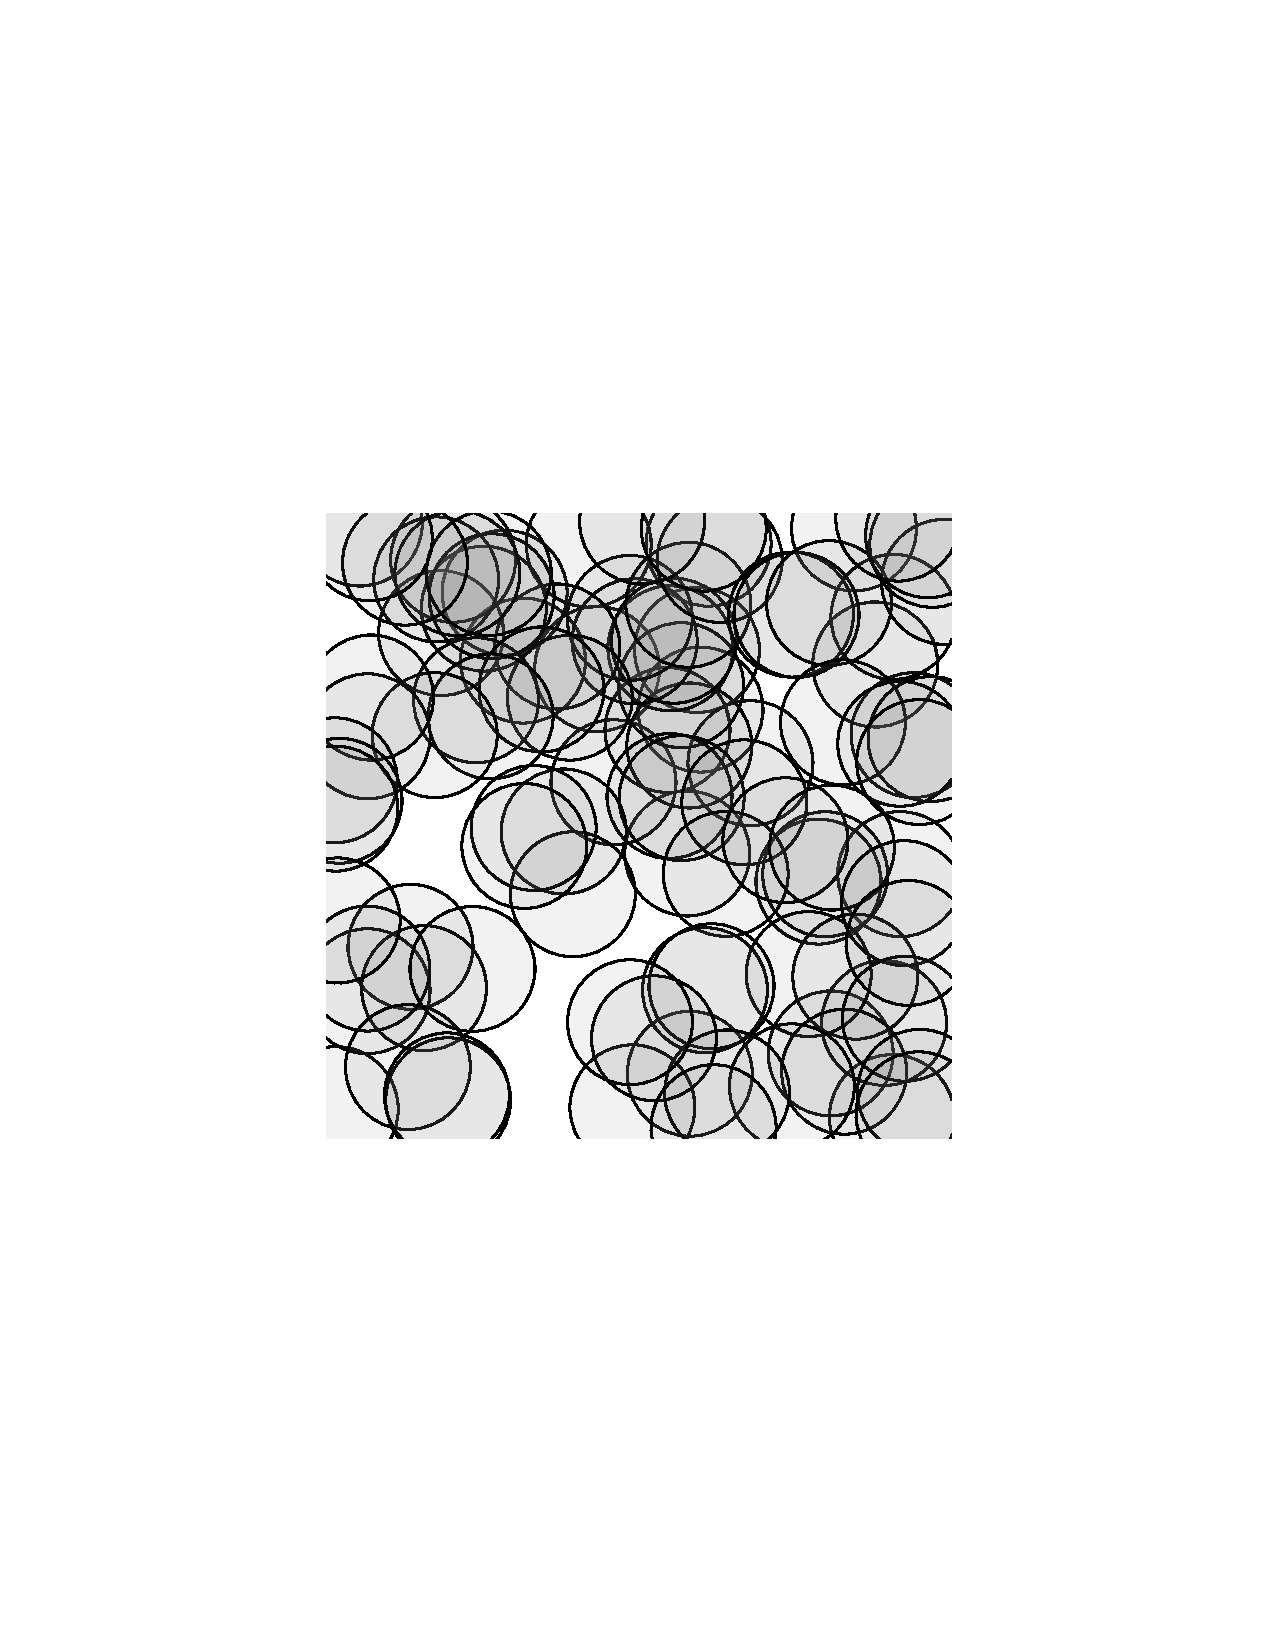
\includegraphics[width=0.3\textwidth]{figures/coverage-30--0-static1}}%
	\subfloat[connectivity]{\label{fig:setup2}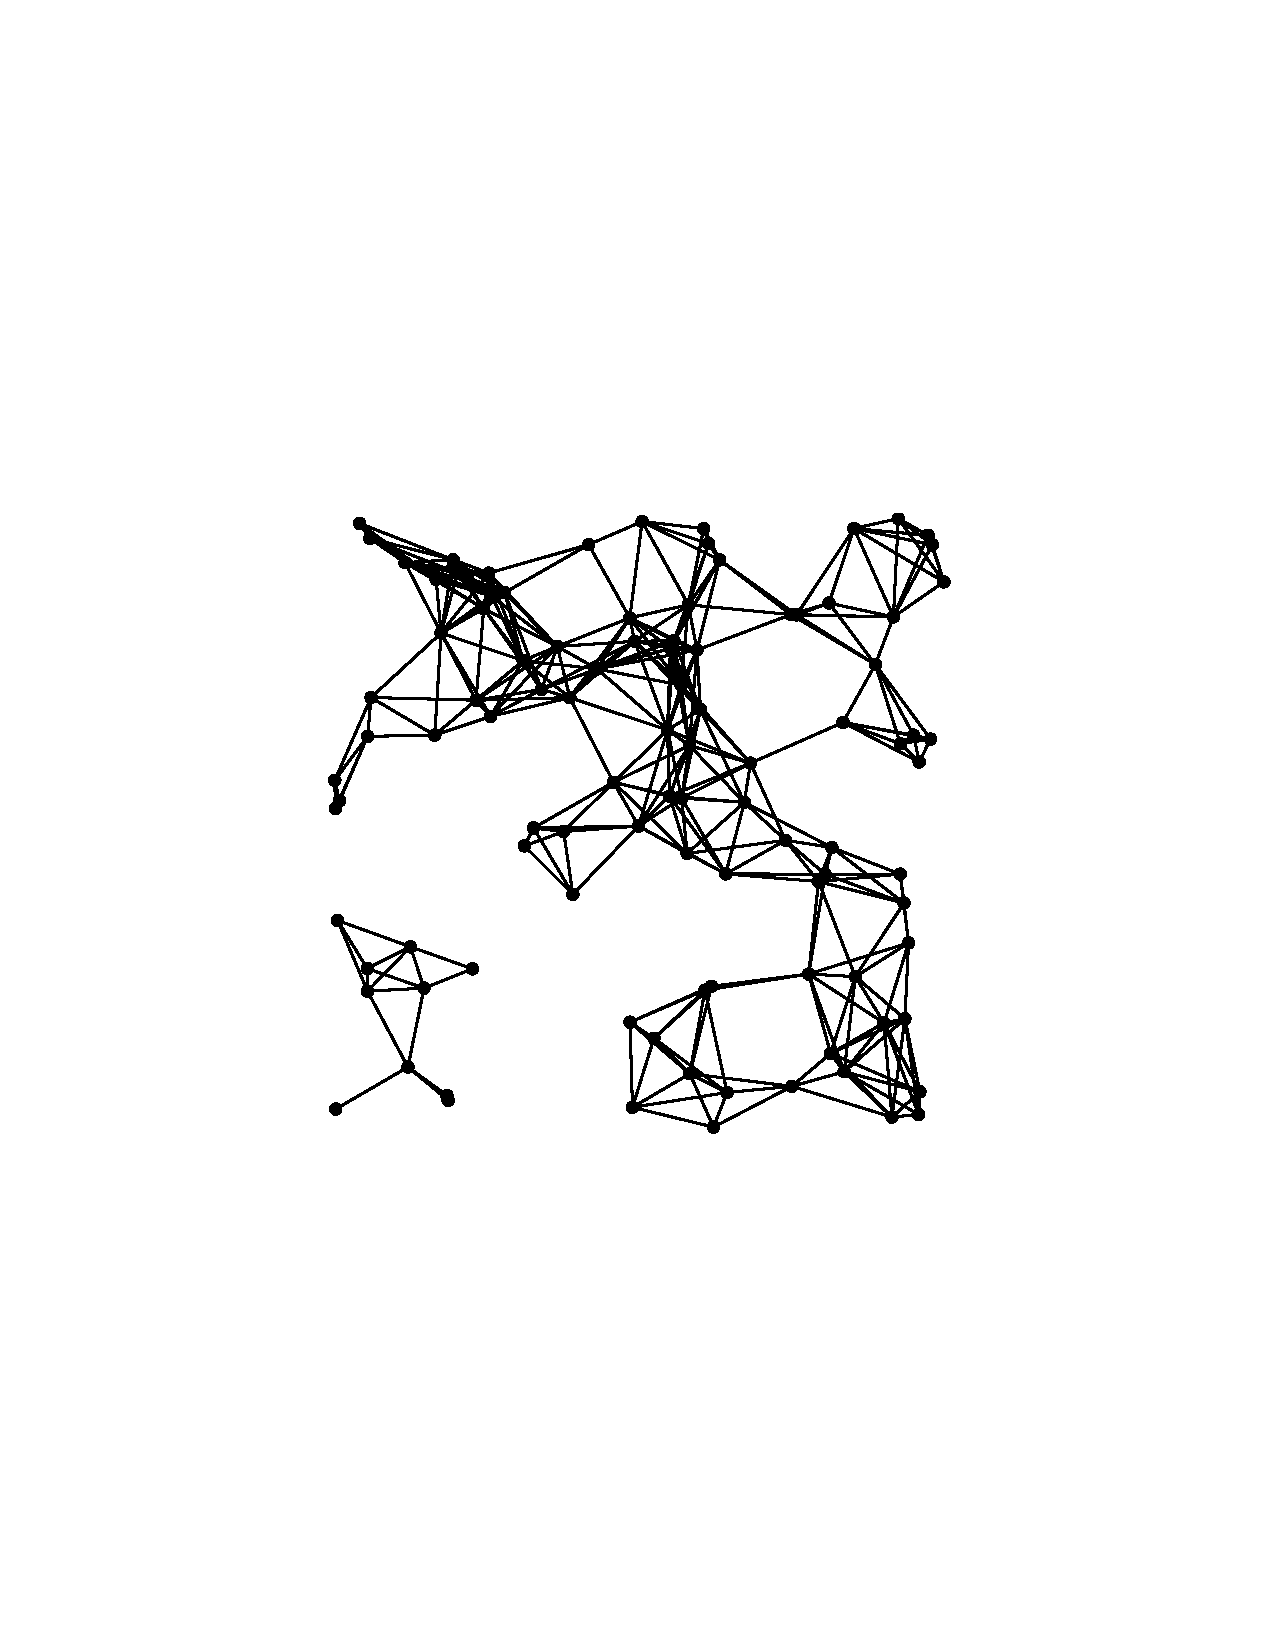
\includegraphics[width=0.3\textwidth]{figures/connectivity-50-0-static1}}
	\caption{Subfigures showing coverage and connectivity for a sample replication at time $t=0$}%
	\label{fig:setups12}%
\end{figure}

\subsection{Tables}

\Cref{tab:SensorNetworkApplications} gives an overview of the discussed application classes.

\begin{table}
	\centering
	\begin{tabular}{>{\raggedright}p{1.8cm}p{5.4cm}p{3.4cm}}
		\toprule
		Class & application examples & lifetime aspects \\
		\midrule
		Critical, coverage & 
				Forest fire detection, flood detection, nuclear/chemical/biological attack detection, battlefield surveillance, intrusion detection & 
				$c_{ca}$/$c_{ct}$/$c_{cb}$, $c_{ln}$, $c_{la}$, $c_{lo}$\\
		Critical, no coverage & 
				Monitoring human physiological data, military monitoring of friendly forces, machine monitoring & 
				$c_{cc}$, $c_{ln}$, $c_{la}$, $c_{lo}$ \\
		Noncritical, coverage & 
				Agriculture, smart buildings, habitat monitoring (sensors monitor the inhabitants in a region) & 
				$c_{ac}$/$c_{tc}$/$c_{bc}$, $c_{cc}$, $c_{sd}$ \\
		Noncritical, no coverage & 
				Home automation, habitat monitoring (sensors are attached to animals and monitor their health and social contacts) & 
				$c_{cc}$, $c_{sd}$ 	\\
		\bottomrule
	\end{tabular}
	\caption{Sensor network applications}
	\label{tab:SensorNetworkApplications}
\end{table}


\subsection{Math}

Simple inlined equations: $\zeta(t) = \min( \zeta_{**}(t))$.
The same in a numbered equation, i.e.\ \cref{eq:zeta}:

\begin{equation}
\zeta(t) = \min( \zeta_{**}(t))
\label{eq:zeta}
\end{equation}

Equations covering multiple lines should be aligned. Note that the numbering is added automatically, independent of whether the equation is actually referenced or not:

\begin{align}
sd_{max} &= max((t_{i+1} - t_i) : \zeta(t_i) < 1, i \in [0, |T|-1]) \\
\psi_{sd}(t) &= \left\{ \begin{array}{cl}
\dfrac{\Delta t_{sd}}{sd_{max}} & sd_{max} > 0 \\
1 & sd_{max} = 0 \\
\end{array} \right.\\
\zeta_{sd}(t) &= \frac{\psi_{sd} - cl_{sd}}{c_{sd} - cl_{sd}}
\end{align}


\subsection{Units}

Units should be set using the \verb|\SI| command: the measurements show that the car was accelerating at \SI{5}{\metre\per\second\squared} until it reached its final speed of \SI{100}{\kilo\metre\per\hour}. Longer unitless numbers or ranges can be typeset using the \verb|\num| and \verb|\numrange| commands, respectively: The number \num{12345678} lies in the range of \numrange{10000000}{20000000}. \Cref{tab:si-in-tables} gives an example of how to typeset numbers and units in tables.

\begin{table}
	\centering
	\begin{tabular}{l>{\raggedright}p{4cm}S[table-text-alignment=left,table-format=1.4e-1]s}
	\toprule
		\multicolumn{2}{l}{factor} & \multicolumn{1}{l}{value} & \multicolumn{1}{c}{unit} \\
	\midrule
		$M$ & vehicle mass & 1.3250e+3 & \kilo\gram \\
		$g$ & gravitational constant & 9.81 & \metre\per\second\squared \\
		$\vartheta$ & road grade & 0 & \degree \\
 		$\alpha$ & & 1.1100 & \gram\per\second \\
 		$\delta$ & & 1.9800e-6 & \gram\per\meter\cubed\second\squared \\
	\bottomrule
	\end{tabular}
	\caption{EMIT factors for a category 9 vehicle}
	\label{tab:si-in-tables}
\end{table}

\subsection{Algorithms}

Based on the periodically transmitted \texttt{hello} messages, the joining node gets information about its physical neighbors and their adjacent nodes. \Cref{alg:H_hello} depicts the handling of \texttt{hello} messages.

\begin{algorithm}
\begin{algorithmic}[1]
\REQUIRE Locally stored state of all neighbors in set $N$
\ENSURE Maintain neighbor set $N$ and set virtual address
\STATE Receive neighbor information from node $N_i$
\IF {$N_i \notin N$}
	\STATE $N \gets N_i$
\ELSE
	\STATE Update $N_i \in N$
\ENDIF
\IF {$P==-1$ AND (Time() $-$ OldTime) $> T_{ps}$}
	\STATE OldTime $\gets$ Time()
	\STATE SetMyPosition()
\ENDIF
\end{algorithmic}
\caption{Handle \texttt{hello} messages}
\label{alg:H_hello}
\end{algorithm}

\subsection{Program Code}

Program code should be omitted, but if absolutely necessary, it should be set as seen in \cref{lst:code}.

\begin{lstlisting}[style=txt,caption=Sample application,label=lst:code]{}
APPLICATION("printU", 192, arg)
{
    // Set Priority
    NutThreadSetPriority(16);
    // main() loop
    for (;;) {
        putchar('U');
        NutSleep(125);
    }
}
\end{lstlisting}


\subsection{References}

To further evaluate the applicability of our definition, we analyzed sensor network applications as surveyed in~\cite{akyildiz2002survey,arampatzis2005survey,khemapach2005survey}. Concerning the importance of different lifetime criteria, most of the application scenarios can be grouped into two main classes with two sub-classes each~\cite{dietrich2009lifetime}.


\subsection{Acronyms}

Acronyms shoud be explained when first used. Latex helps, e.g.\ \acp{MANET} have been frequently used as examples for the development of \ac{WSN} applications.


\subsection{TODOs and FIXMEs}

You can use the the \verb|\TODO| command to add short ``sticky notes'' to your document. 
\TODO{This is what a TODO looks like}
This will also trigger generation of a list-of-TODOs at the end of the document. 
The same goes for the \verb|\FIXME|\FIXME{This is what a FIXME looks like} command.


